% CVPR 2027 author kit (https://github.com/cvpr-org/author-kit), used for a CVPR 2027 workshop submission.
\documentclass[10pt,twocolumn,letterpaper]{article}

\usepackage{cvpr}             % draft: no review banner or line numbers; switch to \usepackage[review]{cvpr} for an anonymous submission
%% This file contains a number of tweaks that are typically applied to the main document.
%% They are not enabled by default, but can be enabled by uncommenting the relevant lines.


%%
%% Official support for 2-column teaser figure
%%
\usepackage{cuted} %< for strip environment

%%
%% For auto-referencing of figures (see fig/teaser.tex and \label{} therein) 
%%
\usepackage{currfile} %< for \currfilebase macro

%%
%% caption and (global) spacing overrides
%%
\usepackage{caption} %< for "\captionof" commands (teaser)
% \setlength{\abovecaptionskip}{.5em} % space above caption
% \setlength{\belowcaptionskip}{1em} % space below caption

%%
%% Inline annotations; for predefined colors, refer to "dvipsnames" in the xcolor package:
%% https://tinyurl.com/overleaf-colors
%%
\newcommand{\red}[1]{{\color{red}#1}}
\newcommand{\todo}[1]{{\color{red}#1}}
\newcommand{\TODO}[1]{\textbf{\color{red}[TODO: #1]}}
%%
%% Disable for camera ready / submission by uncommenting these lines:
%%
% \renewcommand{\TODO}[1]{}
% \renewcommand{\todo}[1]{#1}

%%
%% Work harder in optimizing text layout. Typically shrinks text by 1/6 of page, enable
%% it at the very end of the writing process, when you are just above the page limit.
%%
% \usepackage{microtype}

%%
%% Fine-tune paragraph spacing.
%%
% \renewcommand{\paragraph}[1]{\vspace{.5em}\noindent\textbf{#1.}}

%%
%% Globally adjusts space between figure and caption.
%%
% \setlength{\abovecaptionskip}{.5em}

%%
%% Allows "the use of \paper to refer to the project name"
%% with automatic management of space at the end of the word.
%%
% \usepackage{xspace}
% \newcommand{\paper}{ProjectName\xspace}

%%
%% Commonly used math definitions.
%%
% \DeclareMathOperator*{\argmin}{arg\,min}
% \DeclareMathOperator*{\argmax}{arg\,max}

%%
%% Tighten underline.
%%
% \usepackage{soul}
% \setuldepth{foobar}

%%
%% Fix misplaced line numbers with lineno v5.7/v5.8 (Feb 2026, e.g. early TeX Live 2026 installs).
%% These versions write the column tag outside the column box, so line numbers end up on the
%% wrong side of the column. This backports the fix from lineno v5.9 and does nothing for other
%% lineno versions or in camera-ready mode. Updating TeX Live (tlmgr update --all) also fixes it.
%%
\makeatletter
\@ifpackageloaded{lineno}{\ifdefined\IfFormatAtLeastTF\IfFormatAtLeastTF{2025-06-01}{%
  \@ifpackagelater{lineno}{2026/03/08}{}{\@ifpackagelater{lineno}{2026/02/16}{%
    \RemoveFromHook{build/column/before}[lineno]%
    \AddToHook{build/column/after}{%
      \setbox\@outputbox\vbox to\ht\@outputbox{%
        \boxmaxdepth\@maxdepth
        \protected@write\@auxout{}{%
          \string\def\string\@LN@column{\if@firstcolumn1\else2\fi}}%
        \unvbox\@outputbox}}%
  }{}}}{}\fi}{}
\makeatother


\usepackage{booktabs}
\usepackage{multirow}
\usepackage{makecell}
\usepackage{array}
\usepackage{amsmath,amssymb}
\usepackage{algorithm}
\usepackage{algpseudocode}
\usepackage{enumitem}

\definecolor{cvprblue}{rgb}{0.21,0.49,0.74}
\usepackage[pagebackref,breaklinks,colorlinks,allcolors=cvprblue]{hyperref}

% Pending results: red, so they cannot slip into a submission.
\newcommand{\pend}[1]{\textcolor{red}{[#1]}}
\newcommand{\qq}{\textcolor{red}{\textbf{??}}}
\newcommand{\vv}{\boldsymbol{v}}
\newcommand{\xx}{\boldsymbol{x}}

\def\paperID{****}
\def\confName{CVPR}
\def\confYear{2027}

\title{One Tile Is Enough: Universal Adversarial Perturbations\\on a Tiny Vision-Language Model}

\author{
Author One \quad Author Two \quad Author Three \quad Author Four \quad Author Five \quad El Mahdi El Mhamdi\\[2pt]
{\normalsize \'Ecole polytechnique, Institut Polytechnique de Paris, Palaiseau, France}\\
{\tt\small \{firstname.lastname\}@polytechnique.edu}
}

\begin{document}
\maketitle

\begin{strip}
\centering
\vspace{-3.4em}
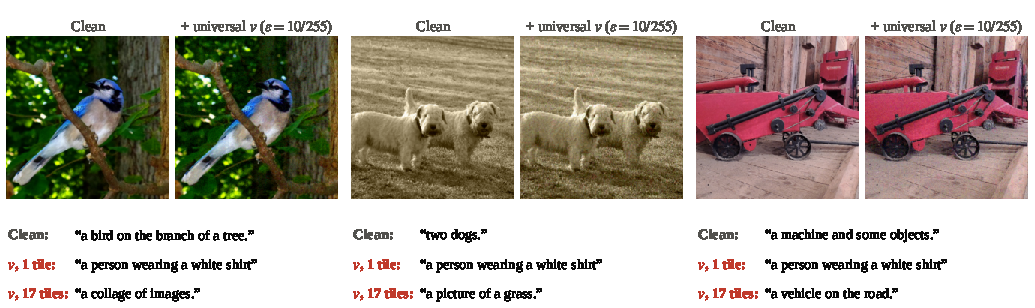
\includegraphics[width=\linewidth]{fig/teaser.pdf}
\captionsetup{hypcap=false}
\captionof{figure}{\textbf{One perturbation, many images.} A single universal perturbation $\vv$ built on 500 images, saved inside each 8-bit image and passed through SmolVLM-256M's own processor, with the resulting captions when the model sees one tile and in its default 17-tile configuration. These three images are the first ones we inspected, and the identical ``white shirt'' caption is \emph{not} representative: over 200 held-out images that phrase appears in about one perturbed caption in six, and 173 of the 200 perturbed captions are distinct (\cref{sec:attack}). What does generalize is the rate: $\vv$ changes 71.5\% (one tile) and 60.5\% (17 tiles) of captions, against at most 4\% for random noise of the same budget.}
\captionsetup{hypcap=true}
\label{fig:teaser}
\end{strip}

\begin{abstract}
Tiny vision-language models (VLMs) now run on phones and embedded devices, where an image goes straight from the camera roll to the model with no server-side filtering in between, yet we are not aware of a study of their robustness to universal adversarial perturbations (UAPs). We study SmolVLM-256M and build a single label-free perturbation by pushing the vision encoder's output tokens away from their clean values, which needs neither labels nor the language model. Built on 500 images and saved inside an ordinary 8-bit image, this perturbation changes 71.5\% of the captions the model writes about unseen images, and 60.5\% in its default tiled configuration, against at most 4\% for random noise of the same $\ell_\infty$ budget, and, added to the preprocessed input, it holds for every prompt we tried, including a closed yes/no question. Looking inside the preprocessing, we find that the attack lives almost entirely in the single downscaled global tile that SmolVLM appends to its 16 detailed tiles, because that view is the only one in which the perturbation keeps its native scale; as a consequence, a perturbation trained on one tile, ignoring the tiling altogether, still breaks the default model. Finally, we benchmark seven defenses, including a tile-aware one that follows from this finding, against fixed, naive adaptive and strong adaptive attackers: every defense except blanking the global tile looks almost perfect against the fixed perturbation (1.5--8.5\% of captions changed), but against the strongest attacker we tested, 29--41\% of captions still change, so no defense is more than partial.
\end{abstract}

\section{Introduction}
\label{sec:intro}

A universal adversarial perturbation is a single, barely visible noise pattern that changes a model's output for most natural images rather than for one image at a time \cite{moosavi2017universal}. Because it is computed once and can be added to any image without access to the model at attack time, it is the cheapest adversarial threat to deploy at scale, and it has been studied extensively for image classifiers and, more recently, for vision-language pre-trained models and large VLMs such as LLaVA, where perturbations computed on the vision encoder alone transfer to the full model \cite{kim2024vevuap,zhang2024etu,fang2024cpgc}.

Tiny VLMs, with a few hundred million parameters, change this picture in three ways that make them worth studying in their own right rather than as a scaled-down copy of large ones. First, they are built to run on the user's device, inside camera, accessibility and assistant applications, so a perturbed image reaches the model directly, without the moderation layers that usually sit in front of a hosted model, and a single perturbation travels with the image wherever it is shared. Second, their weights are public and small enough to download and differentiate through on a free GPU, so an attacker can build a perturbation offline against exactly the model an application ships, and \cref{app:transfer} shows how closely the perturbation is tied to those exact weights. Third, to compensate for that small encoder, tiny VLMs rely on aggressive preprocessing: SmolVLM \cite{marafioti2025smolvlm}, for example, enlarges each image, cuts it into 16 detailed local tiles and appends one downscaled global view, so that the encoder sees the same image at two very different scales. Whether this design changes where a universal perturbation acts, and which cheap defense survives an attacker who knows about it, are questions that results on large VLMs cannot answer.

We answer them on SmolVLM-256M with a label-free version of the original UAP algorithm in which the DeepFool step \cite{moosavi2016deepfool} is replaced by a gradient step on the cosine similarity between clean and perturbed visual tokens. The attack itself is the starting point rather than a contribution, since VEV-UAP \cite{kim2024vevuap} already showed that encoder-only universal perturbations work on large VLMs, and on SmolVLM it works as expected: one perturbation built on 500 ImageNetV2 images at $\epsilon=10/255$ changes \hyperref[tab:attack]{71.5\% of held-out captions, and 60.5\% in the default tiled configuration, against at most 4\% for random noise}, and it carries over to \hyperref[tab:attack]{other prompts, including a yes/no question}. Two measurements make these rates trustworthy. Adding $\vv$ after preprocessing overstates the threat, since it changes \hyperref[tab:attack]{91\% of captions, and the 20 points lost on the way to the real pipeline come entirely from the processor's resize, not from saving the image in 8 bits}; and our caption-change metric agrees with blind human labels on \hyperref[tab:metric]{86\% of decided pairs ($\kappa=0.72$) without ever reporting a change the annotator rejected}, so our rates are conservative. Our main contributions are the following:
\begin{enumerate}[leftmargin=*,itemsep=2pt,topsep=2pt]
  \item \textbf{A causal analysis of where a universal perturbation acts inside a tiled VLM.} We measure the damage on each of the 17 views that SmolVLM's preprocessing creates and introduce a tile-swap test that attributes the caption changes to individual views (\cref{sec:tile}).
  \begin{itemize}[leftmargin=*,itemsep=1pt,topsep=1pt]
    \item We show that the downscaled global tile carries the attack, both in the encoder, \hyperref[fig:tiles]{where its token cosine falls to 0.18 while the local tiles stay near random noise (0.73 against 0.77)}, and in the captions, where \hyperref[tab:swap]{perturbing the global tile alone reproduces 53.5\% of the 60.5\% attack, against 0.5\% for the 16 local tiles}.
    \item We derive the consequence for attackers: tiling does not need to be modelled, since a perturbation built on a single tile already \hyperref[tab:attack]{changes 60.5\% of the default model's captions}, and one trained through the processor \hyperref[tab:swap]{reaches 70.0\%}.
  \end{itemize}
  \item \textbf{A defense benchmark for tiny VLMs under adaptive attackers, including a tile-aware defense.} We propose a defense that randomly resizes only the global tile and evaluate it alongside six other defenses against fixed, naive adaptive and strong adaptive attackers, the last one differentiating through the real processor (\cref{sec:defense}).
  \begin{itemize}[leftmargin=*,itemsep=1pt,topsep=1pt]
    \item We show that evaluating against the fixed perturbation alone is misleading, since it \hyperref[fig:defenses]{makes every defense but one look almost perfect (1.5--8.5\%)}, whereas the strongest attacker we ran \hyperref[tab:defense]{still changes 29--41\% of captions}.
    \item We rank the leading defenses against their own baselines and clean cost, which places the tile-aware defense as \hyperref[tab:defense]{the cheapest on clean captions (2.5\%) but not the most robust (41\% of the attack removed, against 59\% for whole-image resizing)}.
  \end{itemize}
  \item \textbf{A layer-wise view of the attack and of its transfer.} We extend the loss of \cref{eq:loss} to the intermediate states of the encoder and compare every target on SmolVLM-256M, on its 500M sibling and on models outside the family (\cref{sec:layers}).
  \begin{itemize}[leftmargin=*,itemsep=1pt,topsep=1pt]
  \item We show that no single middle layer beats the output, but that combining them does: averaging the loss over layers 3, 6, 9 and the output \hyperref[fig:layers]{changes 83.5\% of captions against 71.0\% for the output alone on the same images} ($p<10^{-4}$), and \hyperref[tab:layers]{72\% against 59\% in the default 17-tile configuration}, because the combined perturbation loses less of its effect through the processor's resize.
  \item We relate transfer to where the encoders diverge: the 256M and 500M encoders are \hyperref[fig:layers]{nearly identical up to layer 3 and unrelated at the output}, so the multi-layer perturbation transfers better to 500M \hyperref[tab:layers]{(44\% against 30.5\%)} and to the original Google SigLIP (up to 48\% against 31\%), whereas nothing transfers to SmolVLM-2.2B or to ImageNet classifiers.
  \end{itemize}
\end{enumerate}

\section{Related work}
\label{sec:related}

\begin{itemize}[leftmargin=*,itemsep=2pt,topsep=2pt]
  \item \textbf{Universal perturbations.}
  \begin{itemize}[leftmargin=*,itemsep=1pt,topsep=1pt]
    \item \emph{Classifiers.} UAPs were introduced by Moosavi-Dezfooli \etal \cite{moosavi2017universal}, who explained them geometrically by the shared normal directions of decision boundaries around natural images.
    \item \emph{Vision-language pre-trained models.} Generator-based UAPs have been proposed against models such as CLIP, ALBEF and BLIP \cite{zhang2024etu,fang2024cpgc}.
    \item \emph{Large VLMs.} VEV-UAP \cite{kim2024vevuap} showed that perturbations computed on the vision encoder alone, without labels or the language model, fool LLaVA-scale models, and that they are strongest when they target middle layers.
    \item \emph{Our position.} Our label-free loss is the simple final-layer baseline of that line of work, applied to a model more than 25 times smaller than LLaVA-7B, where the question is less how to build the strongest perturbation than how the model's own design shapes it; \cref{sec:layers} tests their middle-layer finding on SmolVLM.
  \end{itemize}
  \item \textbf{Defenses and their evaluation.}
  \begin{itemize}[leftmargin=*,itemsep=1pt,topsep=1pt]
    \item \emph{Encoder fine-tuning.} FARE \cite{schlarmann2024fare} fine-tunes a CLIP encoder so that perturbed embeddings stay close to clean ones, and universal adversarial training \cite{shafahi2020uat} trains against a perturbation that evolves with the model.
    \item \emph{Input transformations.} Random resizing and padding \cite{xie2018randomization} is a classic transformation applied to the image before the model sees it.
    \item \emph{Adaptive evaluation.} Athalye \etal \cite{athalye2018obfuscated} and Carlini \etal \cite{carlini2019evaluating} showed how often such defenses collapse once the attacker adapts, which is why every defense here faces an adaptive attacker.
  \end{itemize}
  \item \textbf{Preprocessing as an attack surface.}
  \begin{itemize}[leftmargin=*,itemsep=1pt,topsep=1pt]
    \item \emph{Known weaknesses.} Downscaling can be exploited directly, from image-scaling attacks \cite{xiao2019scaling,quiring2020adversarial} to recent prompt injection through rescaling in multimodal systems \cite{zeeshan2025chameleon}.
    \item \emph{Our position.} Our global-tile finding is a measured, UAP-specific instance of that broader weakness, located inside a VLM's own tiling scheme rather than in an external resizing step.
  \end{itemize}
\end{itemize}

\section{Setting and method}
\label{sec:method}

\textbf{Model and preprocessing.} SmolVLM-256M combines a SigLIP-B/16 encoder \cite{zhai2023siglip} of about 86M parameters, which turns each $512\times512$ tile into 1,024 visual tokens, a pixel-shuffle connector that compresses them to 64 tokens per tile, and a 135M-parameter SmolLM2 language model. With image splitting on, which is the default, the processor enlarges a $512$-pixel image four times, cuts it into 16 local tiles and appends one global tile obtained by shrinking the enlarged image back to 512 pixels (\cref{fig:tiles}a); with splitting off, the model sees a single $512\times512$ tile, which the processor still resizes to 2048 pixels and back with a LANCZOS filter before normalizing it.

\textbf{Threat model.} The attacker's goal is untargeted: make the answer about any image wrong or meaningless, for any prompt, with one perturbation $\vv$ bounded by $\|\vv\|_\infty\le\epsilon$, with $\epsilon=10/255$ unless stated otherwise. The attacker alters the image file before it reaches the model and has white-box access to the vision encoder, but cannot touch the prompt, the language model or the preprocessing. Whenever we evaluate a defense, the attacker also knows the defense and optimizes through it. The defender may transform the image, change how tiles reach the encoder, or fine-tune the encoder, but never retrains the language model. Per-image, targeted, text-side and physical attacks are out of scope.

\textbf{A label-free universal attack.} Since a VLM has no label to flip, we keep the outer loop of the original algorithm, which accumulates updates into $\vv$ and projects it back onto the $\epsilon$-ball, and replace its inner DeepFool step with a gradient step on
\begin{equation}
\min_{\|\vv\|_\infty\le\epsilon}\;\mathbb{E}_{\xx}\Big[\frac{1}{T}\sum_{t=1}^{T}\cos\big(f(\xx)_t,\;f(\mathrm{clip}(\xx+\vv))_t\big)\Big],
\label{eq:loss}
\end{equation}
where $f$ is the encoder's final-layer output and $T=1{,}024$ is the number of tokens per tile (\cref{alg:uap}). Where DeepFool seeks the smallest push across the nearest decision boundary, this step seeks the direction along which the visual tokens of many images move furthest at once, and the projection keeps $\vv$ small, which is the role minimality played in the original method (\cref{app:algo}). Because the loss never sees text, the perturbation is prompt-agnostic by construction.

\begin{algorithm}[t]
\caption{Label-free universal perturbation}
\label{alg:uap}
\small
\begin{algorithmic}[1]
\Require build images $X$, encoder $f$, budget $\epsilon$, passes $E$
\State $\vv \gets \mathbf{0}$; Adam optimizer on $\vv$ with step $\epsilon/10$
\For{$e = 1,\dots,E$}
  \For{each batch $B \subset X$ of 8 images}
    \State $\mathcal{L} \gets \frac{1}{|B|T}\sum_{\xx\in B}\sum_{t} \cos\big(f(\xx)_t, f(\mathrm{clip}(\xx+\vv))_t\big)$
    \State $\vv \gets \mathrm{Adam}(\vv, \nabla_{\vv}\mathcal{L})$ \Comment{push tokens away}
    \State $\vv \gets \mathrm{clip}(\vv, -\epsilon, \epsilon)$ \Comment{project onto the $\ell_\infty$ ball}
  \EndFor
\EndFor
\State \Return $\vv$
\end{algorithmic}
\end{algorithm}

\textbf{Data and evaluation.} We build $\vv$ on the first 500 images of ImageNetV2 matched-frequency \cite{recht2019imagenetv2}, resized to $512\times512$, with 7 to 10 passes that take 15 to 22 minutes on a T4 GPU, and we evaluate on 200 of the next 500, prompting with ``Describe this image in one sentence.'' and decoding greedily, so that any change in the caption comes from the image. Unless stated otherwise, $\vv$ is added to the image, rounded to 8 bits and passed through SmolVLM's own processor, which we call the \emph{real pipeline}. Every attack is compared with random noise of the same budget ($\pm\epsilon$ per pixel), and intervals are 95\% Wilson intervals.

\textbf{When is a caption fooled?} A caption counts as changed when the cosine similarity between the clean and perturbed captions, embedded with all-MiniLM-L6-v2 \cite{reimers2019sbert,wang2020minilm}, falls below 0.5. To check this ruler, one author labelled 60 clean/perturbed pairs, with their condition hidden, as changed in meaning, unchanged, or unsure. On the 44 decided pairs the metric agrees with the annotator on 86.4\% of the pairs ($\kappa=0.72$) and errs only by missing changes, typically fluent captions about a different subject (\cref{tab:metric}, \cref{app:metric}), so all rates below are, if anything, undercounts; we report the stricter 0.7 as a sensitivity check where captions were saved.


\begin{figure*}[t]
\centering
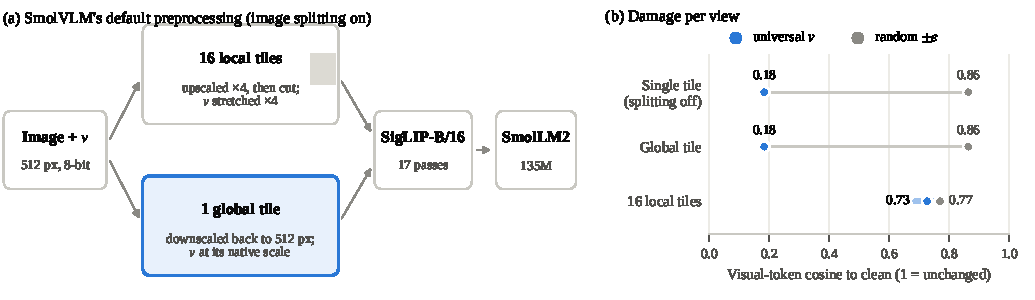
\includegraphics[width=\linewidth]{fig/tiles.pdf}
\caption{\textbf{Where the attack lives.} (a) With image splitting on, the 16 local tiles see the perturbation stretched four times, whereas the global tile sees it at its native scale. (b) Mean visual-token cosine between clean and perturbed tiles on 200 held-out images (the band shows the range over the 16 local tiles): the global tile is damaged exactly as much as the untiled input, since it is the same tile, and the local tiles barely more than by random noise.}
\label{fig:tiles}
\end{figure*}

\section{Results}
\label{sec:results}

\subsection{One perturbation, many images and prompts}
\label{sec:attack}

\cref{tab:attack} summarizes the attack. Added directly to the preprocessed tensor, $\vv$ drives the mean token cosine to $-0.04$, so that perturbed tokens point slightly against their clean versions, and changes 91\% of captions; saved inside the image and passed through the real processor, it still changes 71.5\% with splitting off and 60.5\% with splitting on, while random noise stays at 3--5\%. Separating the two steps of the real pipeline shows where the 20 points go: 8-bit rounding alone changes nothing, since exactly the same 182 captions change with and without it, whereas the processor's resize alone reproduces the whole drop (71.0\%, McNemar $p<10^{-9}$ against tensor space). The round trip keeps 76\% of the perturbation's energy, yet it raises the token cosine from $-0.04$ to 0.18, so the part it removes is the part the encoder reacts to most. Training $\vv$ through the processor, with gradients through an exact copy of the resize, recovers about half of the gap (80.5\%, with 21 captions changing only with the new $\vv$ against 3 only with the old one, $p=0.0003$), and the other half is the cost of the resize itself. We keep the original $\vv$ as the reference for the rest of the paper, so that every defense is measured against the same perturbation. A perturbation built on GoogLeNet with the original algorithm behaves like random noise on SmolVLM (4\%), although it had to be upscaled from 224 to 512 pixels, so we read this only as a sign that a classifier's UAP does not carry over to a VLM encoder.

The perturbation also holds across prompts, which we tested with $\vv$ added to the preprocessed input on 100 images. On three further prompts its rate stays between 80\% and 96\%, and on the closed question ``Is there an animal in this image? Answer yes or no.'' only 28\% of perturbed answers are still a valid ``yes'' or ``no'', against 100\% under random noise, so the model often stops following the format altogether. The short-answer prompt has a high random baseline (28\%), which a comparison of content words reproduces almost exactly (28.3\%), so short answers genuinely vary under small noise rather than reflecting a weakness of the metric.

\begin{table}[t]
\centering
\small
\setlength{\tabcolsep}{2pt}
\begin{tabular}{@{}lcc@{}}
\toprule
Setting / prompt & Universal $\vv$ & Random $\pm\epsilon$ \\
\midrule
\multicolumn{3}{@{}l}{\emph{Describe prompt, 200 images}} \\
Tensor space, 1 tile & 91.0 {\scriptsize[86.2, 94.2]} & 5.0 {\scriptsize[2.7, 9.0]} \\
\quad 8-bit rounding only & 91.0 {\scriptsize[86.2, 94.2]} & -- \\
\quad processor resize only & 71.0 {\scriptsize[64.4, 76.8]} & -- \\
Real pipeline, splitting off & 71.5 {\scriptsize[64.9, 77.3]} & 3.5 {\scriptsize[1.7, 7.0]} \\
Real pipeline, splitting on & 60.5 {\scriptsize[53.6, 67.0]} & 3.0 {\scriptsize[1.4, 6.4]} \\
\midrule
\multicolumn{3}{@{}l}{\emph{$\vv$ trained through the processor, 200 images}} \\
Real pipeline, splitting off & 80.5 {\scriptsize[74.5, 85.4]} & -- \\
Real pipeline, splitting on & 70.0 {\scriptsize[63.3, 75.9]} & -- \\
\midrule
\multicolumn{3}{@{}l}{\emph{Other prompts, tensor space, 100 images}} \\
What is in this image? & 96.0 {\scriptsize[90.2, 98.4]} & 12.0 {\scriptsize[7.0, 19.8]} \\
Main object, few words & 94.0 {\scriptsize[87.5, 97.2]} & 28.0 {\scriptsize[20.1, 37.5]} \\
Animal? yes/no (changed) & 80.0 {\scriptsize[71.1, 86.7]} & 3.0 {\scriptsize[1.0, 8.5]} \\
\bottomrule
\end{tabular}
\caption{Captions changed (\%) by one universal perturbation ($\epsilon=10/255$) and by random noise of the same budget on held-out images. ``Tensor space'' adds $\vv$ after preprocessing; the indented rows apply only one step of the real pipeline; ``real pipeline'' saves $\vv$ in an 8-bit image and uses SmolVLM's processor. Brackets: 95\% Wilson intervals.}
\label{tab:attack}
\end{table}

\textbf{What the damage looks like.} The failure mode depends on how strongly the encoder is hit. In tensor space, where the token cosine is negative, the captions become broken text rather than wrong descriptions, such as digit strings (``2000000000\dots''), loops and fragments (\cref{app:qual}), which suggests that the perturbation erases the image signal and leaves the language model to improvise. Through the real pipeline at $10/255$ the captions become fluent but wrong instead, with a partial attractor towards ``a person wearing a white shirt''. The three examples of \cref{fig:teaser}, where every scene receives that caption, first suggested a collapse onto one caption, but counting all 200 images tells a more modest story: the share of captions mentioning a person doubles, from 14\% to 28\%, the phrase appears in roughly one perturbed caption in six, yet 173 of the 200 perturbed captions remain distinct, so the perturbation pulls a minority of images towards one plausible scene rather than collapsing them all.

\textbf{Budget and visibility.} Training one perturbation per budget shows that the attack grows smoothly with $\epsilon$, from 21.5\% at $4/255$ to 91.5\% at $16/255$, with the steepest gain between 4 and $8/255$, while random noise never exceeds 4\% (\cref{fig:budget}a). The attractor is a middle-budget phenomenon, peaking at $10/255$ and receding at $16/255$, where captions turn back into broken text. PSNR is below the usual 40\,dB rule of thumb at every budget (37.0\,dB at $4/255$, 30.1\,dB at $10/255$), and although the perturbation is hard to notice on textured regions, it is visible on the flattest region we could find even at $4/255$, as structured patterns that include letter-like shapes (\cref{fig:budget}b); we therefore describe it as hard to notice rather than imperceptible.

\begin{figure}[t]
\centering
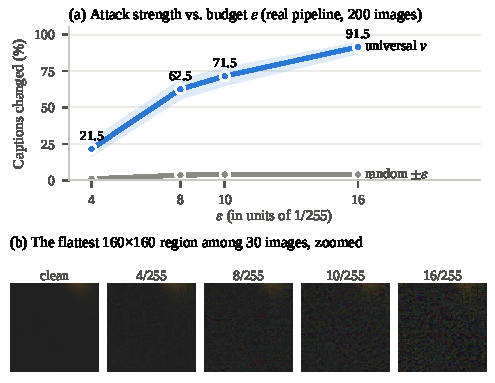
\includegraphics[width=\linewidth]{fig/budget.pdf}
\caption{(a) Captions changed as a function of the budget, through the real pipeline with splitting off; the band is the 95\% interval. (b) The flattest $160\times160$ region found among 30 held-out images, clean and with the perturbation at each budget, shown zoomed: the perturbation is visible on flat regions even at $4/255$.}
\label{fig:budget}
\end{figure}

\subsection{The global tile carries the attack}
\label{sec:tile}

With splitting on, the perturbation still changes most captions (60.5\%), yet the token cosine averaged over the 17 tiles stays at 0.70, against 0.78 for random noise, which means that the damage is concentrated somewhere that the average hides. Measuring each tile separately on the same 200 images locates it (\cref{fig:tiles}b): the global tile reaches a token cosine of 0.18, exactly the value of the single untiled input, which is expected since the two are the same tile, whereas the 16 local tiles average 0.73 (0.69--0.75), close to the 0.77 of random noise.

The reason is geometric. The local tiles are cut from an image enlarged four times, so each of them sees $\vv$ stretched far beyond the scale at which it was optimized, while the global tile shrinks the enlarged image back to 512 pixels and therefore sees $\vv$ almost exactly as it was built. To test whether this damage is what changes the captions, and not only the features, we built the 17 tiles of every clean and perturbed image with the real processor and swapped them before captioning (\cref{tab:swap}). Perturbing only the 16 local tiles changes 1 caption in 200, no more than random noise on all tiles, whereas perturbing only the global tile changes 107, against 121 when every tile is perturbed, so the global tile carries 88\% of the attack on its own, and 96\% for the perturbation trained through the processor. The local tiles matter only in combination: with the original $\vv$, 18 images change only when every tile is perturbed, against 4 that change only with the global tile ($p=0.004$), so local damage can add to a broken global view but cannot break a caption by itself. Since the model always receives that one view, a design meant to give a small model more detail leaves the attack intact, and an attacker can train $\vv$ on a single tile, without modelling the tiling at all, and still change 60.5\% of the default model's captions.

\begin{table}[t]
\centering
\small
\setlength{\tabcolsep}{3pt}
\begin{tabular}{@{}lccc@{}}
\toprule
Tiles perturbed & Original $\vv$ & $\vv$ through processor & Random \\
\midrule
All 17 & 60.5 {\scriptsize[53.6, 67.0]} & 70.0 {\scriptsize[63.3, 75.9]} & 3.0 \\
Global tile only & 53.5 {\scriptsize[46.6, 60.3]} & 67.0 {\scriptsize[60.2, 73.1]} & -- \\
16 local tiles only & 0.5 {\scriptsize[0.1, 2.8]} & 1.0 {\scriptsize[0.3, 3.6]} & -- \\
\bottomrule
\end{tabular}
\caption{Tile swap: captions changed (\%) when only some of the 17 tiles come from the perturbed image (splitting on, 200 held-out images). The global tile alone reproduces 88\% (original $\vv$) and 96\% (trained through the processor) of the full attack; the local tiles alone do nothing.}
\label{tab:swap}
\end{table}

The global view is not only where the vulnerability lives but also a source of context the model relies on: blanking it changes 23\% of clean captions and, once the attacker targets the 16 local tiles directly, raises the attack to 80\%, worse than no defense at all. This is why the defense we derive below perturbs the global tile instead of removing it.



\subsection{Defenses, and the attacker who knows about them}
\label{sec:defense}

\textbf{Defenses.} We test three image transformations, namely JPEG at quality 75, a Gaussian blur with $\sigma=1$ and random resize-and-pad of the whole image (scale 0.8--1.0); two tile-aware defenses, which randomly resize and pad the global tile or blank it; and two ways of fine-tuning only the encoder with a FARE-style feature-anchoring loss, which keeps clean and perturbed tokens close to the original encoder's clean tokens so that the language model still understands them, either on images carrying the fixed $\vv$ (FT-fixed, as in the original paper) or with universal adversarial training, where $\vv$ is updated at every step (FT-UAT).

\textbf{Attackers.} Each defense faces the fixed $\vv$ and a naive adaptive attacker that re-optimizes $\vv$ through an approximation of the defense for three passes with one random draw per step. The leading defenses also face a strong adaptive attacker that forwards every step through SmolVLM's real processor (8-bit rounding, resizing and tile cutting), differentiates through a smooth copy of it (BPDA), whose tiles match the real ones with a token cosine of 0.9975, and averages over random draws of the defense (EOT) for up to 12 passes (\cref{app:defense}).

\begin{figure}[t]
\centering
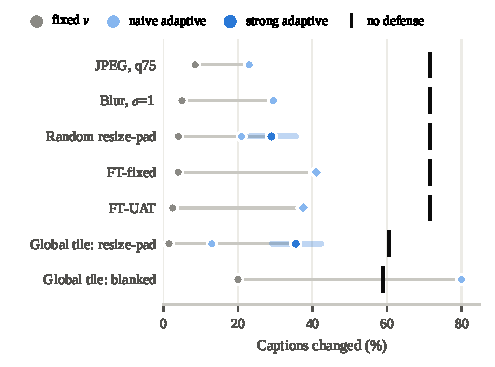
\includegraphics[width=\linewidth]{fig/defenses.pdf}
\caption{Each defense against the fixed perturbation, the naive adaptive attacker and, where run, the strong adaptive attacker (band: 95\% interval), with its own undefended baseline (black tick; 60.5\% for the tile-aware defenses, which run with splitting on). Diamonds: the fine-tuned encoders were attacked with the basic loop of \cref{alg:uap}, without the processor.}
\label{fig:defenses}
\end{figure}

\begin{table}[t]
\centering
\small
\setlength{\tabcolsep}{2.6pt}
\begin{tabular}{@{}lcccc@{}}
\toprule
Defense & \makecell{Clean cost\\0.5\,/\,0.7} & Fixed & \makecell{Strongest\\adaptive} & \makecell{Attack\\cut} \\
\midrule
Random resize-pad & 6.0\,/\,25.0 & 4.0 & 29.0 {\scriptsize[23.2, 35.6]} & 59\% \\
Global tile & 2.5\,/\,\pend{T1} & 1.5 & 35.5 {\scriptsize[29.2, 42.3]} & 41\% \\
FT-UAT & 4.5\,/\,13.5 & 2.5 & 37.5 {\scriptsize[31.1, 44.4]}\rlap{$^\dagger$} & 48\% \\
FT-fixed & 3.0\,/\,8.0 & 4.0 & 41.0 {\scriptsize[34.4, 47.9]}\rlap{$^\dagger$} & 43\% \\
\bottomrule
\end{tabular}
\caption{The four leading defenses against their strongest tested attacker (captions changed, \%, 200 images). ``Attack cut'' is the relative reduction from each defense's own undefended baseline (71.5\%, or 60.5\% for the global tile). $^\dagger$Basic-loop attacker; \pend{M3: strong attacker}.}
\label{tab:defense}
\end{table}

\textbf{Results.} \Cref{fig:defenses} shows the pattern that drives our conclusions. Against the fixed perturbation, every reasonable defense looks almost perfect, cutting the attack from 60--72\% to 1.5--8.5\% at a clean cost of a few percent, but the naive adaptive attacker already recovers 13--30\% against the image transformations and the tile-aware defense, and the strong attacker recovers more again: on the global-tile defense it nearly triples the naive estimate, from 13.0\% to 35.5\%, breaking 50 captions that the naive attacker missed against 5 in the other direction. Its training log shows how it escapes: the defended global tile barely moves (token cosine 0.68 to 0.63) while the local tiles keep degrading (0.36 to 0.25), so the attacker moves onto tiles that are easy to fool once targeted.

\Cref{tab:defense} ranks the four leading defenses against their strongest attacker. Measured against its own baseline, whole-image random resize-and-pad removes about 59\% of the attack and the global-tile defense about 41\%, but their intervals overlap, and the former changes 25\% of clean captions at the stricter 0.7 threshold, against 6\% at 0.5, because it alters many details of normal answers; the global-tile defense is the cheapest on clean captions but not the most robust. Fine-tuning reproduces, on a VLM, the lesson of the original paper's own fine-tuning experiment: both encoders defeat the fixed $\vv$, but a perturbation recomputed against them brings the attack back to 37.5--41\%, and FT-UAT, although much harder to damage in feature space (token cosine 0.68 against 0.36 for FT-fixed), changes almost as many captions, which shows that moderate feature damage is already enough to derail the language model. \pend{M3--M6: strong attacker on FT-fixed and FT-UAT, global-tile attack run to convergence, native 17-tile undefended baseline; update \cref{fig:defenses,tab:defense}.}

\subsection{Middle layers, and how far the perturbation transfers}
\label{sec:layers}

\begin{figure}[t]
\centering
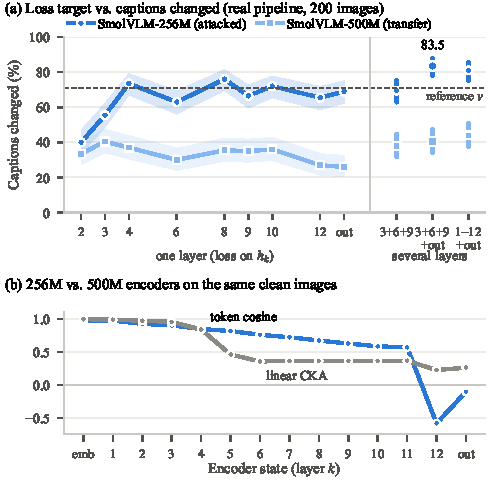
\includegraphics[width=\linewidth]{fig/layers.pdf}
\caption{\textbf{Middle layers and transfer.} (a) Captions changed when the loss targets the state after one encoder layer $k$, the output, or several states at once, on SmolVLM-256M (attacked) and SmolVLM-500M (transfer); bands and bars are 95\% intervals and the dashed line is the reference $\vv$ on 256M. (b) Similarity between the 256M and 500M encoders on the same 50 clean images, state by state ($k=12$ is before the final layer norm, ``out'' after it): the two encoders are nearly identical up to layer 3 and unrelated at the output.}
\label{fig:layers}
\end{figure}

\begin{table}[t]
\centering
\small
\setlength{\tabcolsep}{2pt}
\begin{tabular}{@{}lcccc@{}}
\toprule
Loss target & \makecell{256M\\1 tile} & \makecell{256M\\17 tiles} & \makecell{500M} & \makecell{SigLIP\\(Google)} \\
\midrule
Random $\pm\epsilon$ & 2.5 {\scriptsize[1.1, 5.7]} & 4.0 & 6.5 & 13.8 \\
Output (reference $\vv$) & 71.0 {\scriptsize[64.4, 76.8]} & 59.0 & 30.5 & 31.2 \\
Layer 3 only & 55.5 {\scriptsize[48.6, 62.2]} & 36.0 & 40.5 & 32.6 \\
Layer 8 only & 76.0 {\scriptsize[69.6, 81.4]} & -- & 35.5 & 32.0 \\
Layers 3, 6, 9 & 69.5 {\scriptsize[62.8, 75.5]} & 55.0 & 38.0 & 35.6 \\
Layers 3, 6, 9 + output & \textbf{83.5} {\scriptsize[77.7, 88.0]} & \textbf{72.0} & 40.5 & 40.0 \\
All layers + output & 81.0 {\scriptsize[75.0, 85.8]} & 71.0 & \textbf{44.0} & \textbf{41.8} \\
\bottomrule
\end{tabular}
\caption{Loss target vs.\ attack and transfer (\%, real pipeline). 256M: captions changed on 200 held-out images with one tile (95\% Wilson interval) and on 100 with the default 17 tiles; 500M: captions changed on 200 images; SigLIP (Google): share of 500 images whose zero-shot ImageNet prediction changes. The reference $\vv$ is the perturbation used in the rest of the paper, re-evaluated in the re-run setup (\cref{app:repro}).}
\label{tab:layers}
\end{table}

\textbf{Middle-layer losses.} VEV-UAP \cite{kim2024vevuap} found middle layers to be stronger targets than the output on large VLMs, so we replaced $f$ in \cref{eq:loss} by the residual stream $h_k$ after layer $k$ of the encoder, or averaged the loss over several states, keeping everything else fixed (same 500 build images, $\epsilon=10/255$, 10 passes, one seed per target). No single layer beats the output (\cref{fig:layers}a, \cref{tab:layers}): layers 2 and 3 alone are clearly weaker (40.0\% and 55.5\%), and layers 4 to 12 stay within the output's interval (63--76\% against 69--71\%). Combining the output with middle layers does help: averaging the loss over $h_3$, $h_6$, $h_9$ and the output changes 83.5\% of captions against 71.0\% for the reference $\vv$ on the same images, with 30 images broken only by the combined perturbation against 5 in the other direction (McNemar $p<10^{-4}$), and the gain holds with splitting on (72.0\% against 59.0\% on 100 images). Both parts are needed, since the middle layers alone reach only 69.5\%, and adding every layer brings no further gain (81.0\%). The combined perturbation does not damage the encoder more in tensor space, where the output token cosine is $-0.06$ for both perturbations on 50 images, but it keeps more of that damage through the real pipeline (0.09 against 0.14), whose resize is the step that costs the reference $\vv$ 20 points in \cref{sec:attack}; our reading is that constraining the middle layers, which respond to coarser patterns, keeps $\vv$ from relying on fine details that the resize erases. Targeting $h_6$ alone also produces a much stronger attractor than the output, since 30\% of its captions describe a person in a white shirt and only 102 of 200 are distinct, the closest analogue we found to the dominant labels of \cite{moosavi2017universal}.

\textbf{Transfer.} Passing the same clean images through the 256M and 500M encoders shows where they differ (\cref{fig:layers}b): they are nearly identical up to layer 3 (token cosine $\ge0.90$, linear CKA $\ge0.96$) and then drift apart until their outputs are unrelated (cosine $-0.10$), and their weight matrices tell the same story, differing by 19--26\% in layers 1--8 and by 40--46\% in layers 10--12 (\cref{app:transfer}). Consistently, the output is the target that transfers worst to 500M (26.0\% when re-trained), whereas layer 3 (40.5\%) and the combinations (40.5--44.0\%) transfer best, against 30.5\% for the reference $\vv$ and 6.5\% for random noise. The same pattern holds for the original Google SigLIP-B/16-512 used zero-shot on ImageNet, the checkpoint SmolVLM's encoder starts from: the reference $\vv$ changes 31.2\% of its predictions, the combined perturbations 40.0--41.8\%, and the layer-2 perturbation, built on a layer that fine-tuning moved little, 48.2\%, against 13.8\% for random noise. Beyond that lineage nothing transfers: on SmolVLM-2.2B, whose encoder is a different SigLIP-SO400M, every perturbation stays at or below 14\% (3\% for noise, 100 images), and on ResNet-50 and ViT-B/16 the fooling rate stays within 1--5 points of random noise, which mirrors the GoogLeNet result of \cref{sec:attack} in the other direction.

\section{Discussion and conclusion}
\label{sec:conclusion}

Replacing the label-based inner step with an embedding loss is enough to carry universal perturbations over to a tiny VLM, and one perturbation disrupts most of SmolVLM-256M's answers for any image and any question, through the model's real preprocessing. What changes is everything around the attack: the tiling scheme meant to give a small encoder more detail leaves one downscaled view in which the perturbation keeps its native scale, so that the attacker does not even need to model the tiling, and the leading defenses, the tile-aware one included, looked close to perfect until the attacker adapted, after which 29--41\% of captions still changed. For practitioners deploying tiny VLMs, this means that a perturbation built once on a public encoder is a realistic threat, that robustness should never be reported against a fixed perturbation, and that cheap input transformations buy a partial reduction at a measurable cost on clean answers.

\textbf{Limitations.} All attack and defense results come from one model, one dataset and one seed per perturbation, and they measure whether a caption changed relative to the model's own clean caption rather than whether it became wrong; the metric validation rests on a single annotator; every adaptive number is a lower bound on what an attacker can achieve; the layers of the multi-layer loss were chosen a priori rather than tuned; and every defense was evaluated against the final-layer perturbation only, although the multi-layer one is stronger. Next steps are a second VLM family with a global thumbnail, one without it, and evaluation on COCO. \pend{R1, R3, T3, T4.}

{
    \small
    \bibliographystyle{ieeenat_fullname}
    \bibliography{references}
}

% ---------------------------------------------------------------------------
\clearpage
\appendix
\onecolumn
\section*{Appendix}

\section{From DeepFool to a label-free inner step}
\label{app:algo}

The original algorithm \cite{moosavi2017universal} iterates over images and, for each image $\xx$ that $\vv$ does not yet fool, uses DeepFool to find the smallest additional push that carries $\xx+\vv$ across the nearest decision boundary. For a binary classifier with score $g$, whose boundary is $g=0$, linearizing $g$ around $\xx$ gives the closest point on the boundary through the step
\begin{equation}
r^*(\xx) = -\frac{g(\xx)}{\|\nabla g(\xx)\|_2^2}\,\nabla g(\xx),
\end{equation}
which divides the distance to the boundary by the steepness of the score. In the multi-class case DeepFool computes this distance for the boundary of every competing class, using the difference between that class's score and the current one, picks the closest, and repeats a few times because the boundary is not truly flat. Each minimal push is added to $\vv$, and $\vv$ is projected back onto the $\epsilon$-ball, so that $\vv$ only grows in directions that actually change labels. A VLM has no decision boundary between classes, so our inner step asks a different question, namely which direction moves the visual tokens furthest from their clean values for a batch of images, and answers it with an Adam step on \cref{eq:loss}; \cref{tab:algo} summarizes the differences.

\begin{table}[h]
\centering
\small
\begin{tabular}{@{}>{\raggedright}p{0.22\linewidth}>{\raggedright}p{0.33\linewidth}>{\raggedright\arraybackslash}p{0.36\linewidth}@{}}
\toprule
 & 2017 UAP (DeepFool step) & This work \\
\midrule
One inner step looks for & smallest push across the nearest boundary & largest drop in clean/perturbed token similarity \\
Needs labels & yes & no \\
Images per update & one, only those not yet fooled & a batch of 8, all of them \\
Step size & exact, from the linear approximation & set by Adam ($\epsilon/10$) \\
Keeps $\vv$ small & minimal steps and projection & projection onto the $\epsilon$-ball \\
Success measured by & label flips (fooling rate) & token cosine and caption change \\
\bottomrule
\end{tabular}
\caption{The 2017 inner step and ours.}
\label{tab:algo}
\end{table}

\section{Metric validation details}
\label{app:metric}

From the 1,600 clean/perturbed caption pairs of the budget sweep we removed the 377 identical pairs and drew 60 of the rest, one per image, stratified by a character-overlap score so that borderline cases are well represented, then shuffled them and hid their condition. The annotator marked 30 pairs as changed, 14 as unchanged and 16 as unsure. On the 44 decided pairs the metric ranks the pairs exactly as the annotator does, since every pair judged unchanged scores at least 0.755 and every pair judged changed at most 0.652, so agreement depends only on the threshold (\cref{tab:metric}). The labels also confirm the attack independently of the metric: 27 of 37 universal-perturbation pairs were judged changed, including all 10 at $16/255$, against 3 of 23 random-noise pairs. The unsure pairs are mostly detail-level changes under random noise or at the smallest budget, where, without the image, one cannot tell whether a new detail is wrong or merely different; 15 of them score above 0.5, and 6 below 0.7, so the stricter threshold starts counting them. Because the sample is stratified, these agreement rates describe the metric's behaviour around the threshold rather than its agreement on all pairs, and a second annotator would turn the check into a proper agreement study. \pend{T1: overlap-score definition, reweighting to the 1,600 pairs, second annotator.}

\begin{table}[h]
\centering
\small
\setlength{\tabcolsep}{4pt}
\begin{tabular}{@{}ccccc@{}}
\toprule
Threshold & Agreement & $\kappa$ & Over-calls & Misses \\
\midrule
0.3 & 70.5\% & 0.45 & 0 & 13 \\
\textbf{0.5} & \textbf{86.4\%} & \textbf{0.72} & \textbf{0} & \textbf{6} \\
0.6 & 97.7\% & 0.95 & 0 & 1 \\
0.7 & 100\% & 1.00 & 0 & 0 \\
\bottomrule
\end{tabular}
\caption{The caption-change metric against blind human labels on 44 decided pairs. ``Over-calls'': the metric reports a change the annotator rejected; ``Misses'': the reverse.}
\label{tab:metric}
\end{table}

\begin{table}[h]
\centering
\small
\begin{tabular}{@{}cccccc@{}}
\toprule
$\epsilon$ & Universal $\vv$ & Random $\pm\epsilon$ & Token cosine ($\vv$) & ``Person''/``white shirt'' captions & PSNR \\
\midrule
4/255 & 21.5 [16.4, 27.7] & 1.0 & 0.623 & 14\% & 37.0\,dB \\
8/255 & 62.5 [55.6, 68.9] & 3.5 & 0.291 & 22\% & 32.0\,dB \\
10/255 & 71.5 [64.9, 77.3] & 4.0 & 0.142 & 28\% & 30.1\,dB \\
16/255 & 91.5 [86.8, 94.6] & 4.0 & $-0.054$ & 18\% & 26.4\,dB \\
\bottomrule
\end{tabular}
\caption{Budget sweep (real pipeline, splitting off, 200 images; token cosine on 50 images). The random baseline at $10/255$ (4.0\%) differs from \cref{tab:attack} (3.5\%) because the sweep draws its own noise vector.}
\label{tab:eps}
\end{table}

\section{Transfer across the SmolVLM family}
\label{app:transfer}

We tested the perturbation built on SmolVLM-256M on SmolVLM-500M, which uses the same SigLIP-B/16 architecture with a larger language model, and on SmolVLM-2.2B, which uses SigLIP-SO400M at 384 pixels (real pipeline, splitting off). The perturbation changes 31.0\% [25.0, 37.7] of captions on 500M against 10.0\% for random noise, and 7.0\% [3.4, 13.7] on 2.2B against 3.0\%, within the noise of 100 images. The encoder-level numbers explain most of the drop on 500M: its token cosine under $\vv$ is 0.706 instead of 0.142, and a direct comparison of the two encoders shows that all 197 tensors share names and shapes but none is identical, with a median relative difference of 1.9\%, so the two encoders start from the same checkpoint and were fine-tuned separately. That median understates the gap, however, because 123 of the 197 tensors are biases and layer-norm parameters that barely move (about 1\%): the 74 weight matrices, which hold 99.9\% of the parameters, differ by 26\% in median, and most in the last layers (\cref{sec:layers}). A perturbation is therefore closely tuned to the exact weights it was built on, although the caption-level drop also mixes in 500M's own connector and language model, and the 2.2B result mixes in the rescaling of $\vv$ to 384 pixels. \pend{R2: transfer controls, e.g.\ the 500M encoder inside the 256M model.}

\section{Qualitative examples in tensor space}
\label{app:qual}

\begin{figure}[h]
\centering
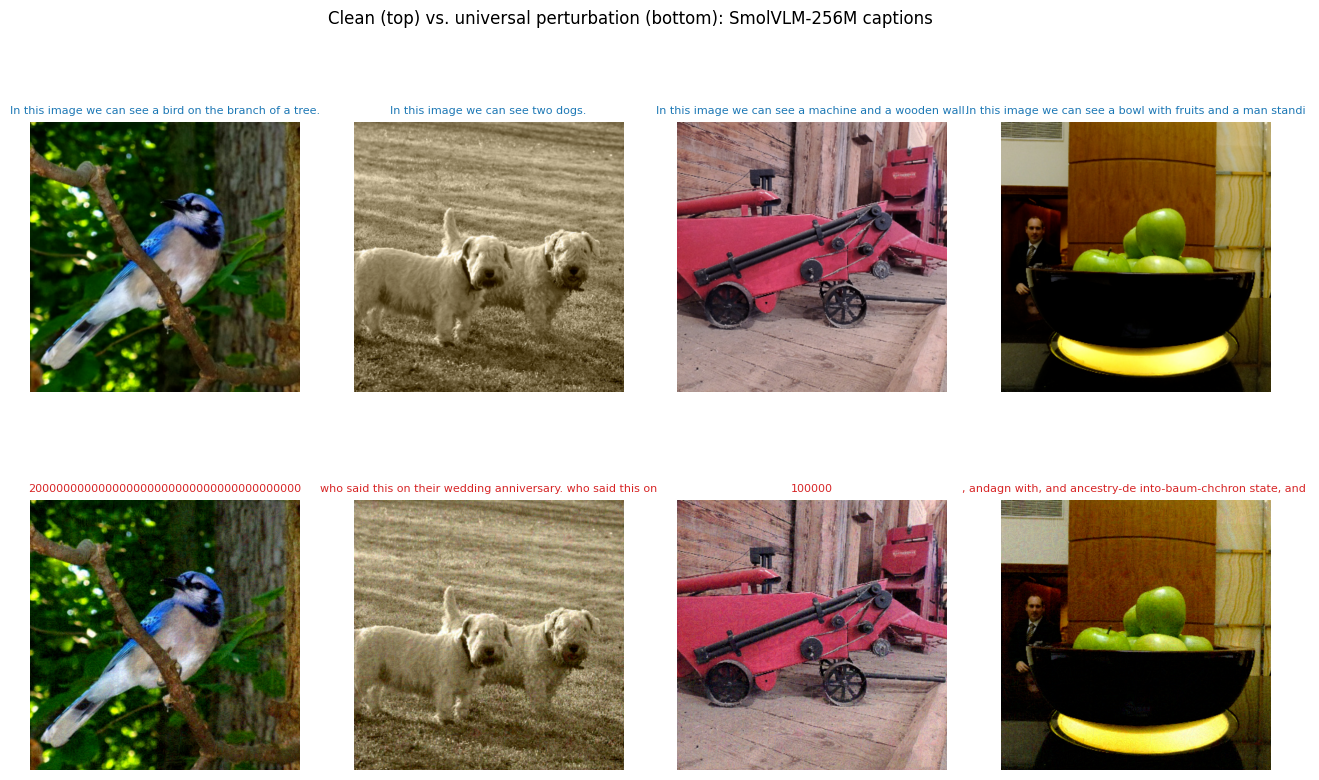
\includegraphics[width=0.85\linewidth]{fig/examples_tensor.png}
\caption{Clean images (top) and the same images with the universal perturbation added in tensor space (bottom), with SmolVLM-256M's captions: the perturbed captions are broken text rather than wrong descriptions.}
\label{fig:qual-tensor}
\end{figure}

\section{Defense and attacker details}
\label{app:defense}

\textbf{Defenses.} All test-time defenses act on the 8-bit perturbed image and are measured against the defended clean captions. Random resize-and-pad rescales the image by a factor drawn in $[0.8,1.0]$ with bilinear resizing and pads it on a mid-gray canvas; the global-tile variant does the same to the global tile only; the blanked defense replaces the global tile by a uniform gray image passed through the processor, since an all-zero tile is treated as padding and dropped. FT-fixed and FT-UAT fine-tune only the encoder for 3 epochs (learning rate $10^{-5}$, batch 8, anchor weight 1.0) on the same 500 build images the attacker uses, and both drift little from the original encoder (clean-token cosine 0.971 and 0.953). \Cref{tab:defense-all} gives every number behind \cref{fig:defenses}.

\textbf{Attackers.} Every adaptive attacker starts from the fixed $\vv$. The naive attacker runs 3 passes with one random draw of the defense per step, uses a straight-through gradient for JPEG and, for tile-aware defenses, approximates the tiling by bicubic upscaling. The strong attacker forwards every step through SmolVLM's real processor and back-propagates through our smooth copy of it, averages over 2 random draws of the defense per step, splits its loss equally between the global tile and 3 sampled local tiles per step, and runs up to 12 passes. On random resize-and-pad it converged (29.0\% after 8 passes against 28.0\% after 6, loss 0.543 to 0.541); on the global-tile defense it was still improving slowly (30.5\% after 6 passes, 35.5\% after 12, loss 0.459 to 0.443), so that number is a lower bound. At 12 passes its perturbation is more effective against the defended model (35.5\%) than against the undefended one (29.5\%), because it has specialized to the defended pipeline. \pend{M4: more local tiles per step and 4 draws, run to convergence.}

\begin{table}[h]
\centering
\small
\begin{tabular}{@{}lccccccc@{}}
\toprule
Defense & Tiles & $n$ & Baseline & Clean cost 0.5\,/\,0.7 & Fixed $\vv$ & Naive adaptive & Strong adaptive \\
\midrule
JPEG, quality 75            & 1  & 200 & 71.5 & 3.0\,/\,--   & 8.5 & 23.0 & \pend{R4} \\
Gaussian blur, $\sigma=1$   & 1  & 200 & 71.5 & 6.0\,/\,--   & 5.0 & 29.5 & -- \\
Random resize-and-pad       & 1  & 200 & 71.5 & 6.0\,/\,25.0 & 4.0 & 21.0 & 29.0 [23.2, 35.6] \\
FT-fixed (encoder)          & 1  & 200 & 71.5 & 3.0\,/\,8.0  & 4.0 & 41.0 [34.4, 47.9]$^\dagger$ & \pend{M3} \\
FT-UAT (encoder)            & 1  & 200 & 71.5 & 4.5\,/\,13.5 & 2.5 & 37.5 [31.1, 44.4]$^\dagger$ & \pend{M3} \\
Global tile: resize-and-pad & 17 & 200 & 60.5 & 2.5\,/\,\pend{T1} & 1.5 & 13.0 & 35.5 [29.2, 42.3] \\
Global tile: blanked        & 17 & 100 & 59.0 & 23.0\,/\,--  & 20.0 & 80.0 & -- \\
\bottomrule
\end{tabular}
\caption{All defenses (captions changed, \%, $\epsilon=10/255$). $^\dagger$Basic-loop attacker of \cref{alg:uap}, 7 passes, without 8-bit rounding or the processor.}
\label{tab:defense-all}
\end{table}

\section{Reproducibility}
\label{app:repro}

Images live in $[0,1]$ pixel space and are clamped there, $\epsilon$ is expressed in pixel units, and normalization happens inside $f$. The attacked representation is the encoder's \texttt{last\_hidden\_state}, after its final layer norm and before the connector. Random noise is a single Rademacher vector ($\pm\epsilon$ per pixel) shared by all images. Evaluation subsets are nested prefixes of held-out images 500--999 in a fixed random permutation of ImageNetV2 matched-frequency. All results use \texttt{transformers==5.22.1} and \texttt{torch==2.14.1} on a single T4 GPU; we observed different numbers with other library versions, so the version should be pinned. The experiments of \cref{sec:layers} were run separately, with \texttt{transformers==5.5.4} and \texttt{torch==2.6.0} on an RTX 4050, training $\vv$ in bfloat16 and evaluating in float32; in that setup the reference $\vv$ changes 71.0\% of captions instead of 71.5\%, 199 of the 200 clean captions are identical word for word, and \cref{tab:layers} compares every target with the reference $\vv$ re-evaluated there. The code, results and perturbations are in \texttt{smol\_exp/13\_middle\_layer\_loss\_and\_transfer.ipynb} and \texttt{smol\_exp/reruns\_code/}. \pend{Code release link.}

\section{Hypotheses that did not survive}
\label{app:revisions}

Several early readings changed under harsher tests, and we report them because each changed a conclusion. A token-cosine threshold of 0.9 looked like a useful ``embedding fooling rate'' until random noise passed it for 91.6\% of images. The 91\% of the first run became 71.5\% once the perturbation went through the real pipeline. A collapse onto one ``dominant caption'', seen in three out of three examples, turned out to be a partial attractor affecting about one image in six. The 256M and 500M encoders, which we assumed shared their weights, differ by 1.9\% in median over all tensors, and that median was itself misleading, since their weight matrices differ by 26\%. The perturbation, judged barely perceptible on grass, is visible on flat regions. Finally, the global-tile defense, which held a naive adaptive attacker to 10\% on 100 images, reached 35.5\% against a stronger attacker on 200, and the idea of removing the global tile backfired because the model needs its context.

\end{document}
